\documentclass{article}

\usepackage{graphicx}
\usepackage{tikz}
\usepackage{tikzsymbols}
\usetikzlibrary{calc,patterns,shapes.geometric}
\pagestyle{empty}
\usepackage[margin=0pt]{geometry}
\geometry{papersize={14in,12in}}

\def\centerarc[#1](#2)(#3:#4:#5){\draw[#1] ($(#2)+({#5*cos(#3)},{#5*sin(#3)})$) arc (#3:#4:#5);}

\begin{document}
	\begin{figure}
		\centering
		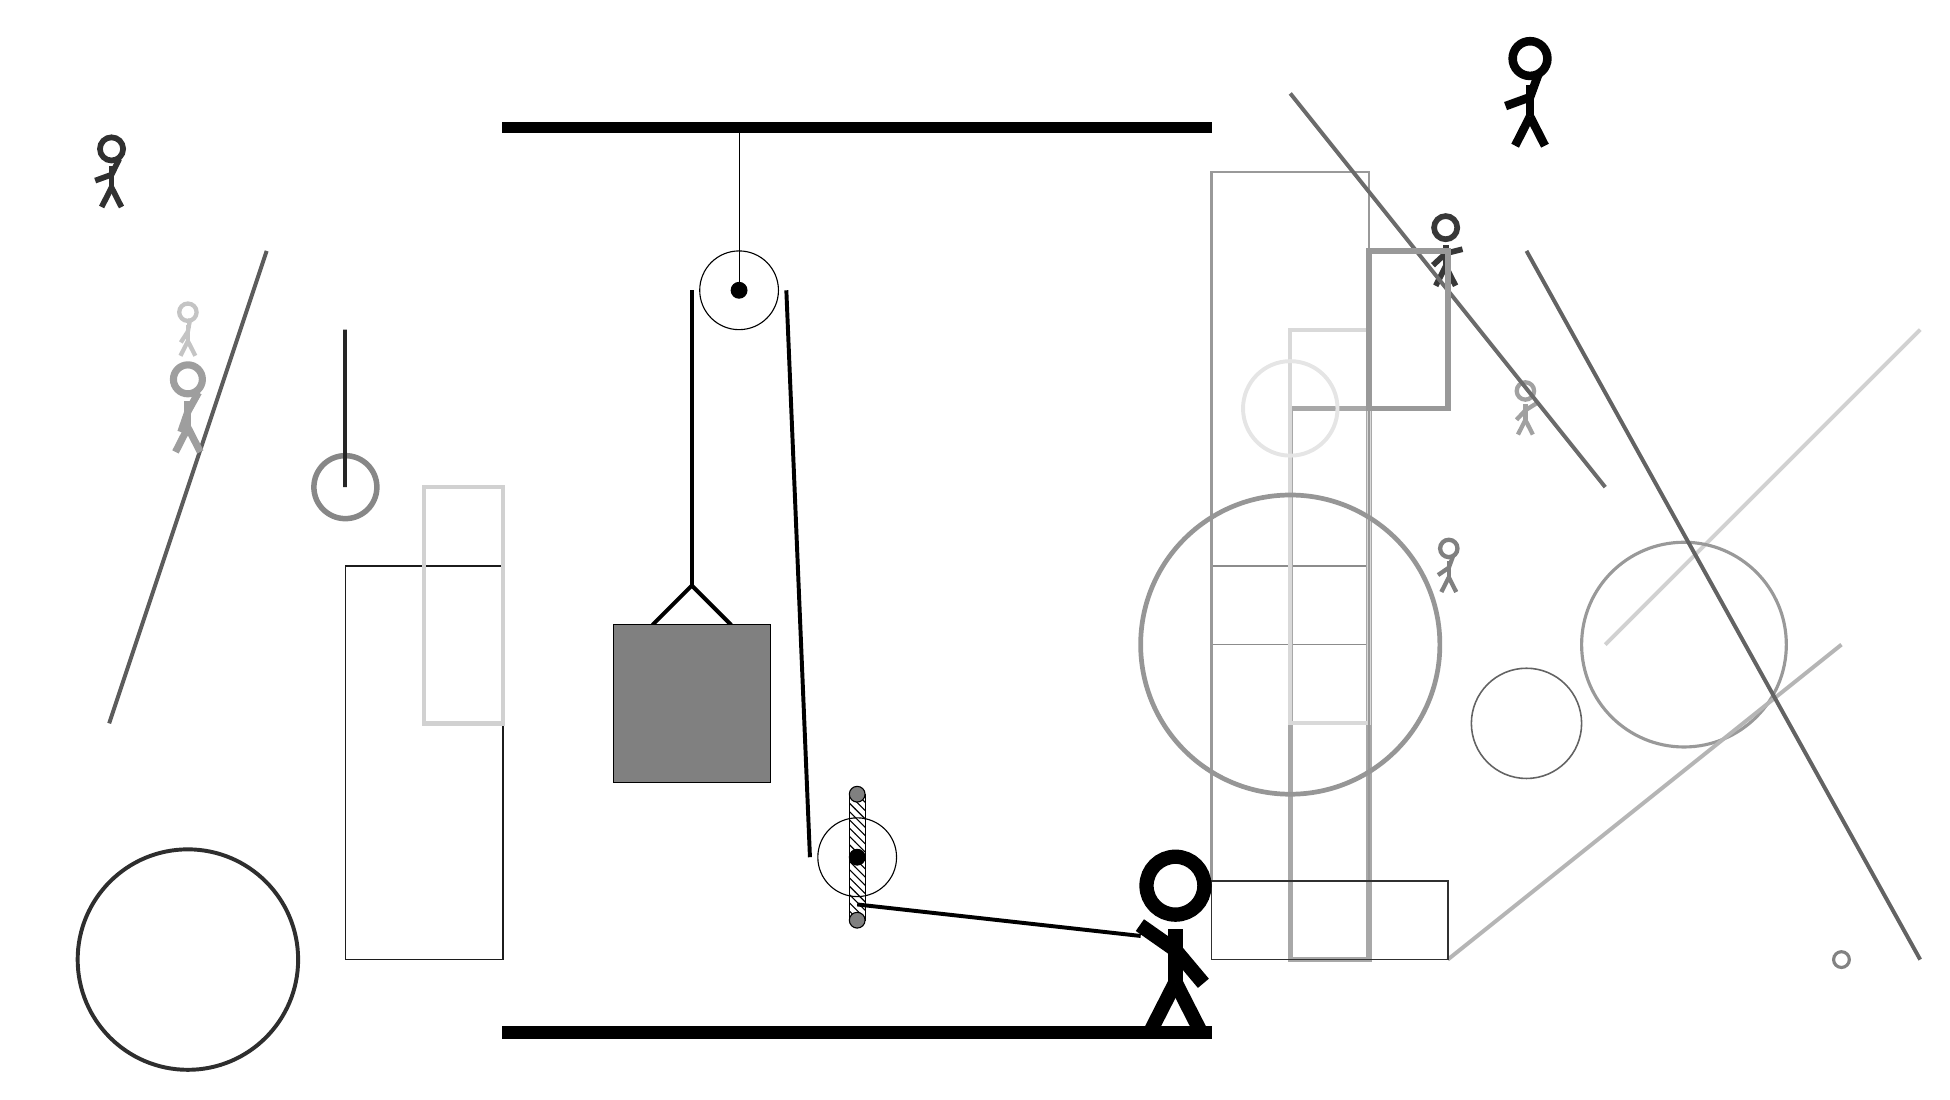
\begin{tikzpicture}
			%%%%% START %%%%%
			
			\draw[fill=black] (-2, 11.5) rectangle (7, 11.625);
			
			\draw (1, 9.5) circle (0.5);
			\draw[fill=black] (1, 9.5) circle (0.1);
			\draw (1, 11.5) -- (1, 9.5);
			
			\draw[fill=white](2.5, 2.3) circle (0.5);
			\draw[fill=black] (2.5, 2.3) circle (0.1);
			\draw[pattern=north west lines, pattern color=black] (2.4, 3.1) rectangle (2.6, 1.5);
			\draw[fill=black!50] (2.5, 3.1) circle (0.1);
			\draw[fill=black!50] (2.5, 1.5) circle (0.1);
			
			\draw[line width=0.5mm] (-0.1, 5.25) -- (0.4, 5.75) -- (0.9, 5.25);
			\draw[fill=black!50] (-0.6, 5.25) rectangle (1.4, 3.25);
			
			\draw[line width=0.2mm, color=black!45] (9, 5) rectangle (7, 6);
			
			\node[line width=0.7mm, color=black!99] at (11, 12) {\Strichmaxerl[6][20][70]};
			\draw [line width=0.2mm, color=black!61](11, 4) circle (0.7);
			\draw[line width=0.7mm, color=black!34] (8, 8) rectangle (9, 1);
			\draw[line width=0.5mm, color=black!15] (9, 4) rectangle (8, 9);
			
			\draw [line width=0.5mm, color=black!82](-6, 1) circle (1.4);
			
			\draw[line width=0.3mm, color=black!40] (7, 11) rectangle (9, 2);
			\draw [line width=0.4mm, color=black!49](15, 1) circle (0.1);
			\node[line width=0.4mm, color=black!50] at (10, 6) {\Strichmaxerl[3][34][70]};
			
			\node[line width=0.4mm, color=black!81] at (-7, 11) {\Strichmaxerl[4][20][64]};
			\draw[line width=0.2mm, color=black!89] (-4, 6) rectangle (-2, 1);
			\draw[line width=0.5mm, color=black!18](12, 5) -- (16, 9);
			\node[line width=0.4mm, color=black!37] at (11, 8) {\Strichmaxerl[3][47][32]};
			
			\draw [line width=0.6mm, color=black!41](8, 5) circle (1.9);
			\node[line width=0.7mm, color=black!23] at (-6, 9) {\Strichmaxerl[3][57][80]};
			\draw[line width=0.5mm, color=black!64](-7, 4) -- (-5, 10);
			
			\node[line width=0.7mm, color=black!78] at (10, 10) {\Strichmaxerl[4][43][14]};
			\draw[line width=0.6mm, color=black!18] (-3, 7) rectangle (-2, 4);
			\draw [line width=0.5mm, color=black!10](8, 8) circle (0.6);
			\draw [line width=0.7mm, color=black!46](-8, 4) circle (0.0);
			\draw[line width=0.5mm, color=black!58](8, 12) -- (12, 7);
			
			\draw [line width=0.4mm, color=black!40](13, 5) circle (1.3);
			\draw[line width=0.7mm, color=black!40] (9, 10) rectangle (10, 8);
			\node[line width=0.4mm, color=black!38] at (-6, 8) {\Strichmaxerl[5][71][61]};
			\draw[line width=0.5mm, color=black!29](10, 1) -- (15, 5);
			
			\draw[line width=0.5mm, color=black!61](11, 10) -- (16, 1);
			
			\draw[line width=0.2mm, color=black!81] (7, 1) rectangle (10, 2);
			\draw [line width=0.7mm, color=black!47](-4, 7) circle (0.4);
			\draw[line width=0.5mm, color=black!85] (-4, 7) rectangle (-4, 9);
			
			\draw[line width=0.5mm] (0.4, 9.5) -- (0.4, 5.75);
			\centerarc[line width=0.5mm](1, 9.5)(0:180:0.6);
			\draw[line width=0.5mm](1.6, 9.5) -- (1.9, 2.3);
			\centerarc[line width=0.5mm](2.5, 2.3)(180:270:0.6);
			\draw[line width=0.5mm](2.5, 1.7) -- (6.1, 1.3);
			
			\node at (6.5, 1.2) {\Strichmaxerl[10][-35][-50]};
			
			\draw[fill=black] (-2, 0) rectangle (7, 0.15);
			
			%%%%% END %%%%%
		\end{tikzpicture}
	\end{figure}	
\end{document}